\documentclass{article}
\usepackage{hyperref}
\usepackage{fancyhdr}
\usepackage{tikz}
\usepackage{multicol}
\usepackage{pgf}
\usepackage{graphicx} 
\usepackage{array}
\usepackage{mdframed}
\usepackage[left=1in,right=1in,top=1in, bottom=1in]{geometry}
\usepackage{float}
\usepackage{color}
\usepackage{xcolor}
\usepackage[utf8]{inputenc}
\usepackage[arabic]{babel}
\usepackage{polyglossia}
\usepackage{fontspec}
\setmainlanguage{arabic}
\newfontfamily\arabicfont[Script=Arabic]{Tajawal}
\usepackage{tocloft}
\addtolength{\cftsecnumwidth}{12pt}
\addtolength{\cftsubsecnumwidth}{12pt}
\setlength{\cftsubsecindent}{30pt}
\usepackage{endnotes}
\usepackage{scrextend}
\usepackage[utf8]{inputenc}
\usepackage{url}
\usepackage{paralist}
\newcolumntype{R}[1]{>{\let\newline\\\arraybackslash\hspace{0pt}}m{#1}}

\usepackage{authblk}
\usepackage{tablefootnote}
\usepackage{todonotes}
\usepackage{lscape}
\usepackage{chronology}
\usepackage{enumitem, amssymb}
\usepackage{booktabs} 
\usepackage{dcolumn}
\definecolor{abblue}{RGB}{30,150,186}
\definecolor{abblueD}{RGB}{44,143,159}
\definecolor{aborange}{RGB}{223,109,33}

\pagestyle{fancy}
\fancyhf{}
\renewcommand\headrule{}
\fancyhead[L]{\color{gray}\footnotesize{الباروميتر العربي} \\
	\color{gray}\footnotesize{كتاب البيانات}}
\cfoot{\color{gray}\footnotesize{الباروميتر العربي}}
\rfoot{\color{gray}\footnotesize{ \thepage}}
\usepackage{background}
\hypersetup{colorlinks=false,pdfborder=0 0 0,citebordercolor={0 0 0}}


\begin{document}

	\newpage
	\backgroundsetup{
		scale=1,
		color=black,
		opacity=1,
		angle=0,
		contents={%
			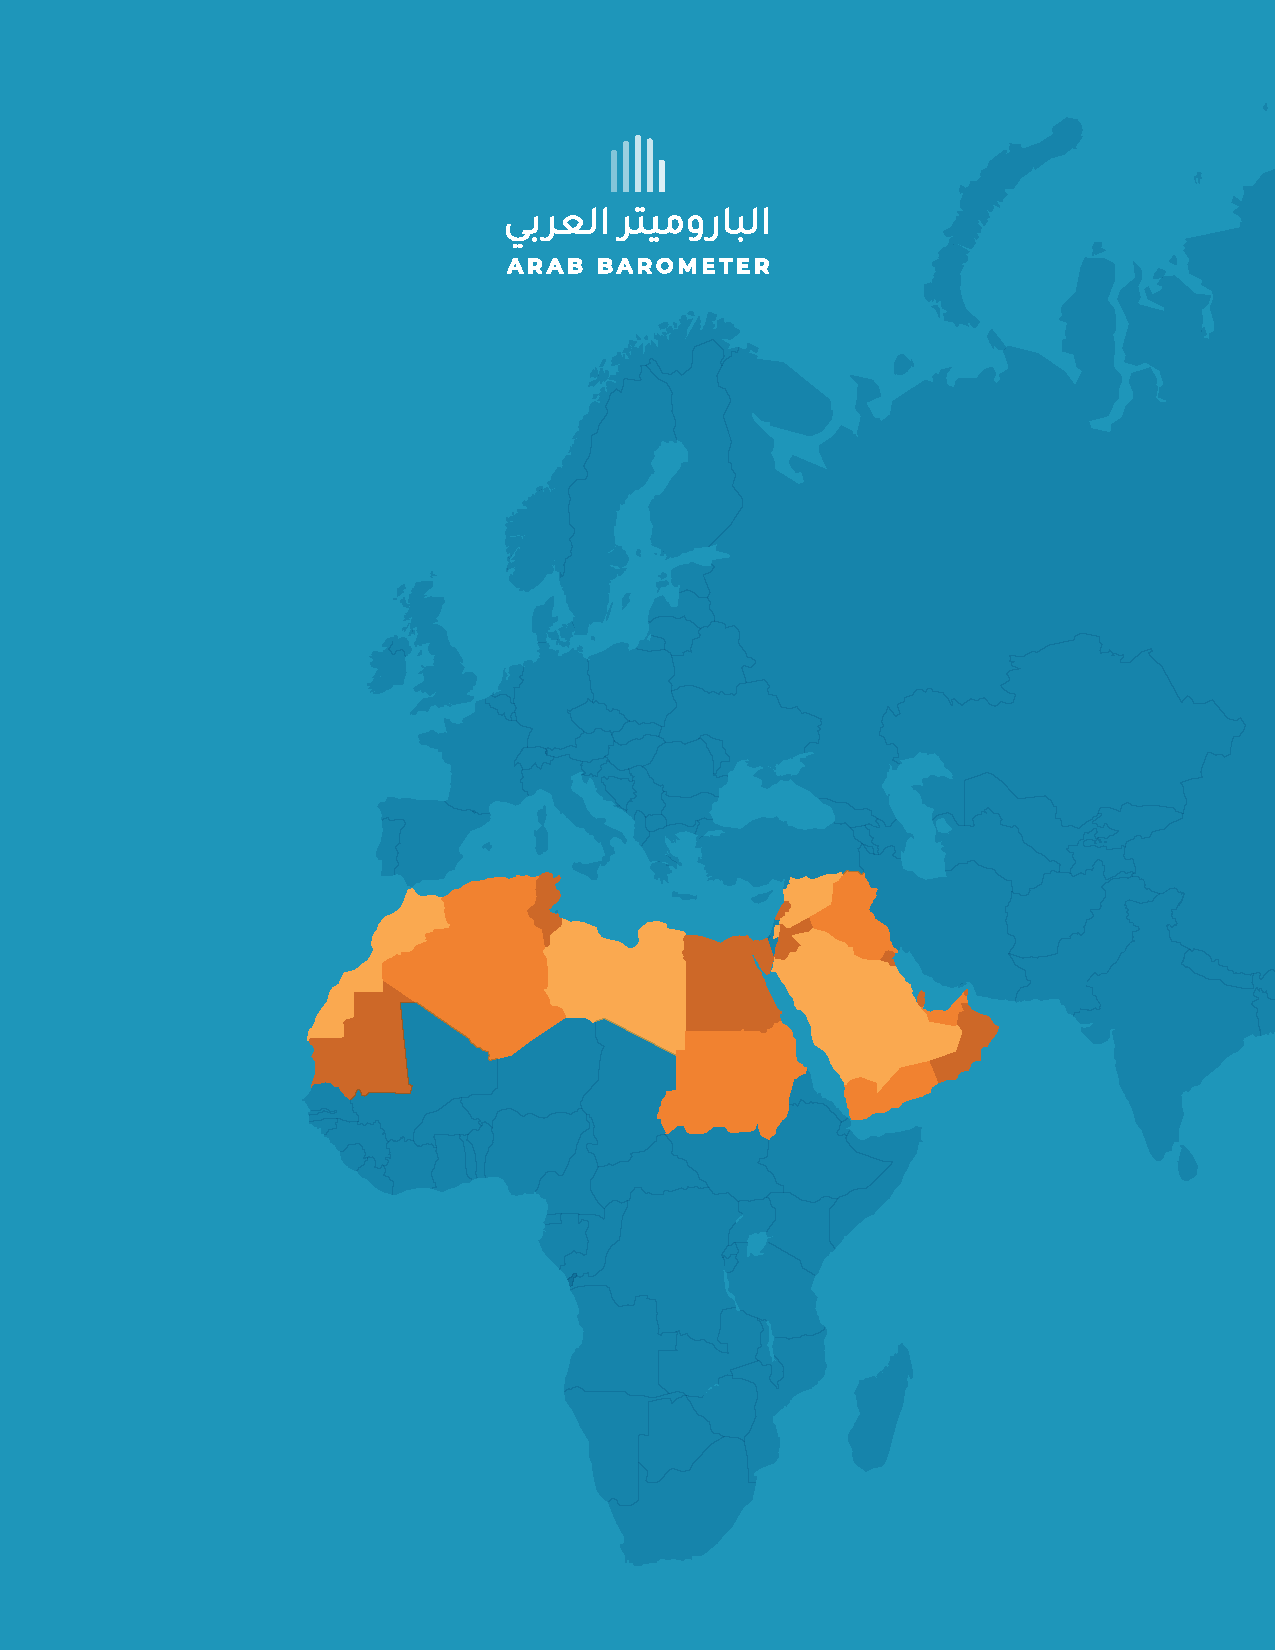
\includegraphics[width=\paperwidth,height=\paperheight]{AB_FrontCover.pdf}
		}%
	}
	\newgeometry{left=1in,right=1in,top=1in, bottom=1in}
	\pagestyle{empty} 
	\vspace*{2in}
	\begin{center}
		\color{white}\Large\textbf{طلب للبيانات،} \\
		\vspace*{0.5in}
		\color{white}\large{٢٠١٩} \\
		\vspace*{4in}
		\color{white}\large{الديمقراطية حول العالم العربي-الدورة الخامسة} \\
	\end{center}
	%%%%%%%%%%%%%%%%%%%%%%%%%%%%
	\newpage\backgroundsetup{contents={}}
	\color{gray}
	%%%%%%%%%%%%%%%%%%%%%%%%%%%%
	\color{gray}
	\pagestyle{fancy}



الملخص التنفيذي
المغرب بلد منقسم بين جيلين. فالجيل الأكبر من المغاربة يحتفظ بالثقة في مؤسسات الدولة، في حين أن الجيل الأصغر من المغاربة يعاني من تزايد الإحباط إزاء نقص الفرص الاقتصادية والسياسية. ما زال المغرب بلدًا مستقرًا، لكن حالة الغضب في أوساط الشباب لا تنبئ بالخير، لا سيما مع انتشار الاضطرابات في عدد من دول المنطقة. يجب أن يكون بين أولويات الحكومة الأساسية تلبية احتياجات وبواعث قلق هذا الجيل الصاعد. 

وفي نظر المواطنين، فإن التحديات الكبيرة التي تواجه المغرب تشمل الاقتصاد وجودة الخدمات العامة. والأغلبية العظمى من المغاربة تقول أيضاً إن الفساد قائم في مؤسسات الدولة، وإن كانت نسبة مؤيدي هذا الرأي قد تراجعت في السنوات الأخيرة، وربما يعكس هذا جهود معالجة مشكلة الفساد. 

إن عدم القدرة على حل هذه المشكلات المزمنة لها أيضاً تبعات على الحكومة. فمستويات الثقة في المؤسسات السياسية متدنية وآخذة في التراجع، لا سيما في أوساط الجيل الشاب. على ذلك، فما زالت الثقة عالية في الجيش والشرطة والقضاء.

تدفع هذه التحديات نحو نصف المغاربة إلى التفكير في الهجرة من بلدهم، بما يشمل 7 من كل 10 أشخاص بين 18 و29 عاماً. ومن المقلق بصورة خاصة أن من يرغبون في الهجرة هم أيضاً أصحاب التعليم العالي، الذين يمكن أن يكونوا قادة المستقبل في المغرب. ويسعى أكثر الراغبين في الهجرة إلى البحث عن فرص في أوروبا – ويُرجح أن يكون السبب هو قربها جغرافياً من المغرب – وإن كانت الأغلبية تقول إنها لن تغادر المغرب إلا بعد الحصول على تصاريح قانونية بالهجرة. كما أن الجيل الشاب يبتعد عن الدين، على الأقل مقارنة بالأجيال الأكبر. فشخص واحد من بين كل 4 أشخاص في الشريحة العمرية 18-29 عاماً وصف نفسه بأنه متدين، مقارنة بثلثي من تبلغ أعمارهم 60 عاماً فأكثر. وبالمثل، فإن دعم الإسلام السياسي انحسر بحدة في المغرب، لا سيما في أوساط الشباب.

هذه هي بعض النتائج الأساسية لاستطلاع للرأي العام لعينة ممثلة لمستوى الدولة، أجراها الباروميتر العربي في المغرب في الفترة من أكتوبر/تشرين الأول إلى ديسمبر/كانون الأول 2018. وقد تم إجراء الاستطلاع عن طريق مقابلات شخصية وجهاً لوجه مع 2400 شخص، في بيوت المبحوثين، وكان هامش الخطأ ±2 بالمئة وكانت نسبة الاستجابة 55 بالمئة.

%%%%%%%%%%%%%%%%%%%%%%%%%%%%%%%%%%%  
\newpage


\begin{figure}[H]
\centering
\caption{}
\includegraphics[scale=.75]{'vtext'_trend (1).png}
\label{fig:my_label}
\end{figure}

\begin{figure}[H]
\centering
\caption{}
\includegraphics[scale=.75]{Algeria_trend.png}
\label{fig:my_label}
\end{figure}

\begin{figure}[H]
\centering
\caption{}
\includegraphics[scale=.75]{Egypt_trend.png}
\label{fig:my_label}
\end{figure}

\begin{figure}[H]
\centering
\caption{}
\includegraphics[scale=.75]{Iraq_trend.png}
\label{fig:my_label}
\end{figure}

\begin{figure}[H]
\centering
\caption{}
\includegraphics[scale=.75]{Jordan_trend.png}
\label{fig:my_label}
\end{figure}

\begin{figure}[H]
\centering
\caption{}
\includegraphics[scale=.75]{Lebanon_trend.png}
\label{fig:my_label}
\end{figure}

\begin{figure}[H]
\centering
\caption{}
\includegraphics[scale=.75]{Morocco_trend.png}
\label{fig:my_label}
\end{figure}

\begin{figure}[H]
\centering
\caption{}
\includegraphics[scale=.75]{Q511_overall.pdf}
\label{fig:my_label}
\end{figure}

\begin{figure}[H]
\centering
\caption{}
\includegraphics[scale=.75]{R511_overall.pdf}
\label{fig:my_label}
\end{figure}

\begin{figure}[H]
\centering
\caption{}
\includegraphics[scale=.75]{R515A1_age.pdf}
\label{fig:my_label}
\end{figure}

\begin{figure}[H]
\centering
\caption{}
\includegraphics[scale=.75]{R515A1_edu.pdf}
\label{fig:my_label}
\end{figure}

\begin{figure}[H]
\centering
\caption{}
\includegraphics[scale=.75]{R515A1_gender.pdf}
\label{fig:my_label}
\end{figure}

\begin{figure}[H]
\centering
\caption{}
\includegraphics[scale=.75]{R515A1_income.pdf}
\label{fig:my_label}
\end{figure}

\begin{figure}[H]
\centering
\caption{}
\includegraphics[scale=.75]{R515A1_overall.pdf}
\label{fig:my_label}
\end{figure}

\begin{figure}[H]
\centering
\caption{}
\includegraphics[scale=.75]{R515A2_age.pdf}
\label{fig:my_label}
\end{figure}

\begin{figure}[H]
\centering
\caption{}
\includegraphics[scale=.75]{R515A2_edu.pdf}
\label{fig:my_label}
\end{figure}

\begin{figure}[H]
\centering
\caption{}
\includegraphics[scale=.75]{R515A2_gender.pdf}
\label{fig:my_label}
\end{figure}

\begin{figure}[H]
\centering
\caption{}
\includegraphics[scale=.75]{R515A2_income.pdf}
\label{fig:my_label}
\end{figure}

\begin{figure}[H]
\centering
\caption{}
\includegraphics[scale=.75]{R515A2_overall.pdf}
\label{fig:my_label}
\end{figure}

\begin{figure}[H]
\centering
\caption{}
\includegraphics[scale=.75]{R515A3_age.pdf}
\label{fig:my_label}
\end{figure}

\begin{figure}[H]
\centering
\caption{}
\includegraphics[scale=.75]{R515A3_edu.pdf}
\label{fig:my_label}
\end{figure}

\begin{figure}[H]
\centering
\caption{}
\includegraphics[scale=.75]{R515A3_gender.pdf}
\label{fig:my_label}
\end{figure}

\begin{figure}[H]
\centering
\caption{}
\includegraphics[scale=.75]{R515A3_income.pdf}
\label{fig:my_label}
\end{figure}

\begin{figure}[H]
\centering
\caption{}
\includegraphics[scale=.75]{R515A3_overall (1).pdf}
\label{fig:my_label}
\end{figure}

\begin{figure}[H]
\centering
\caption{}
\includegraphics[scale=.75]{R515A4_age.pdf}
\label{fig:my_label}
\end{figure}

\begin{figure}[H]
\centering
\caption{}
\includegraphics[scale=.75]{R515A4_edu.pdf}
\label{fig:my_label}
\end{figure}

\begin{figure}[H]
\centering
\caption{}
\includegraphics[scale=.75]{R515A4_gender.pdf}
\label{fig:my_label}
\end{figure}

\begin{figure}[H]
\centering
\caption{}
\includegraphics[scale=.75]{R515A4_income.pdf}
\label{fig:my_label}
\end{figure}

\begin{figure}[H]
\centering
\caption{}
\includegraphics[scale=.75]{R515A4_overall (1).pdf}
\label{fig:my_label}
\end{figure}

\begin{figure}[H]
\centering
\caption{}
\includegraphics[scale=.75]{R516A1_age.pdf}
\label{fig:my_label}
\end{figure}

\begin{figure}[H]
\centering
\caption{}
\includegraphics[scale=.75]{R516A1_edu.pdf}
\label{fig:my_label}
\end{figure}

\begin{figure}[H]
\centering
\caption{}
\includegraphics[scale=.75]{R516A1_overall.pdf}
\label{fig:my_label}
\end{figure}

\begin{figure}[H]
\centering
\caption{}
\includegraphics[scale=.75]{R516A2_age.pdf}
\label{fig:my_label}
\end{figure}

\begin{figure}[H]
\centering
\caption{}
\includegraphics[scale=.75]{R516A2_edu.pdf}
\label{fig:my_label}
\end{figure}

\begin{figure}[H]
\centering
\caption{}
\includegraphics[scale=.75]{R516A2_overall.pdf}
\label{fig:my_label}
\end{figure}

\begin{figure}[H]
\centering
\caption{}
\includegraphics[scale=.75]{R516A3_age.pdf}
\label{fig:my_label}
\end{figure}

\begin{figure}[H]
\centering
\caption{}
\includegraphics[scale=.75]{R516A3_edu.pdf}
\label{fig:my_label}
\end{figure}

\begin{figure}[H]
\centering
\caption{}
\includegraphics[scale=.75]{R516A3_overall.pdf}
\label{fig:my_label}
\end{figure}

\begin{figure}[H]
\centering
\caption{}
\includegraphics[scale=.75]{Sudan_trend.png}
\label{fig:my_label}
\end{figure}

\pagestyle{empty}
\backgroundsetup{
	scale=1,
	color=black,
	opacity=1,
	angle=0,
	contents={%
		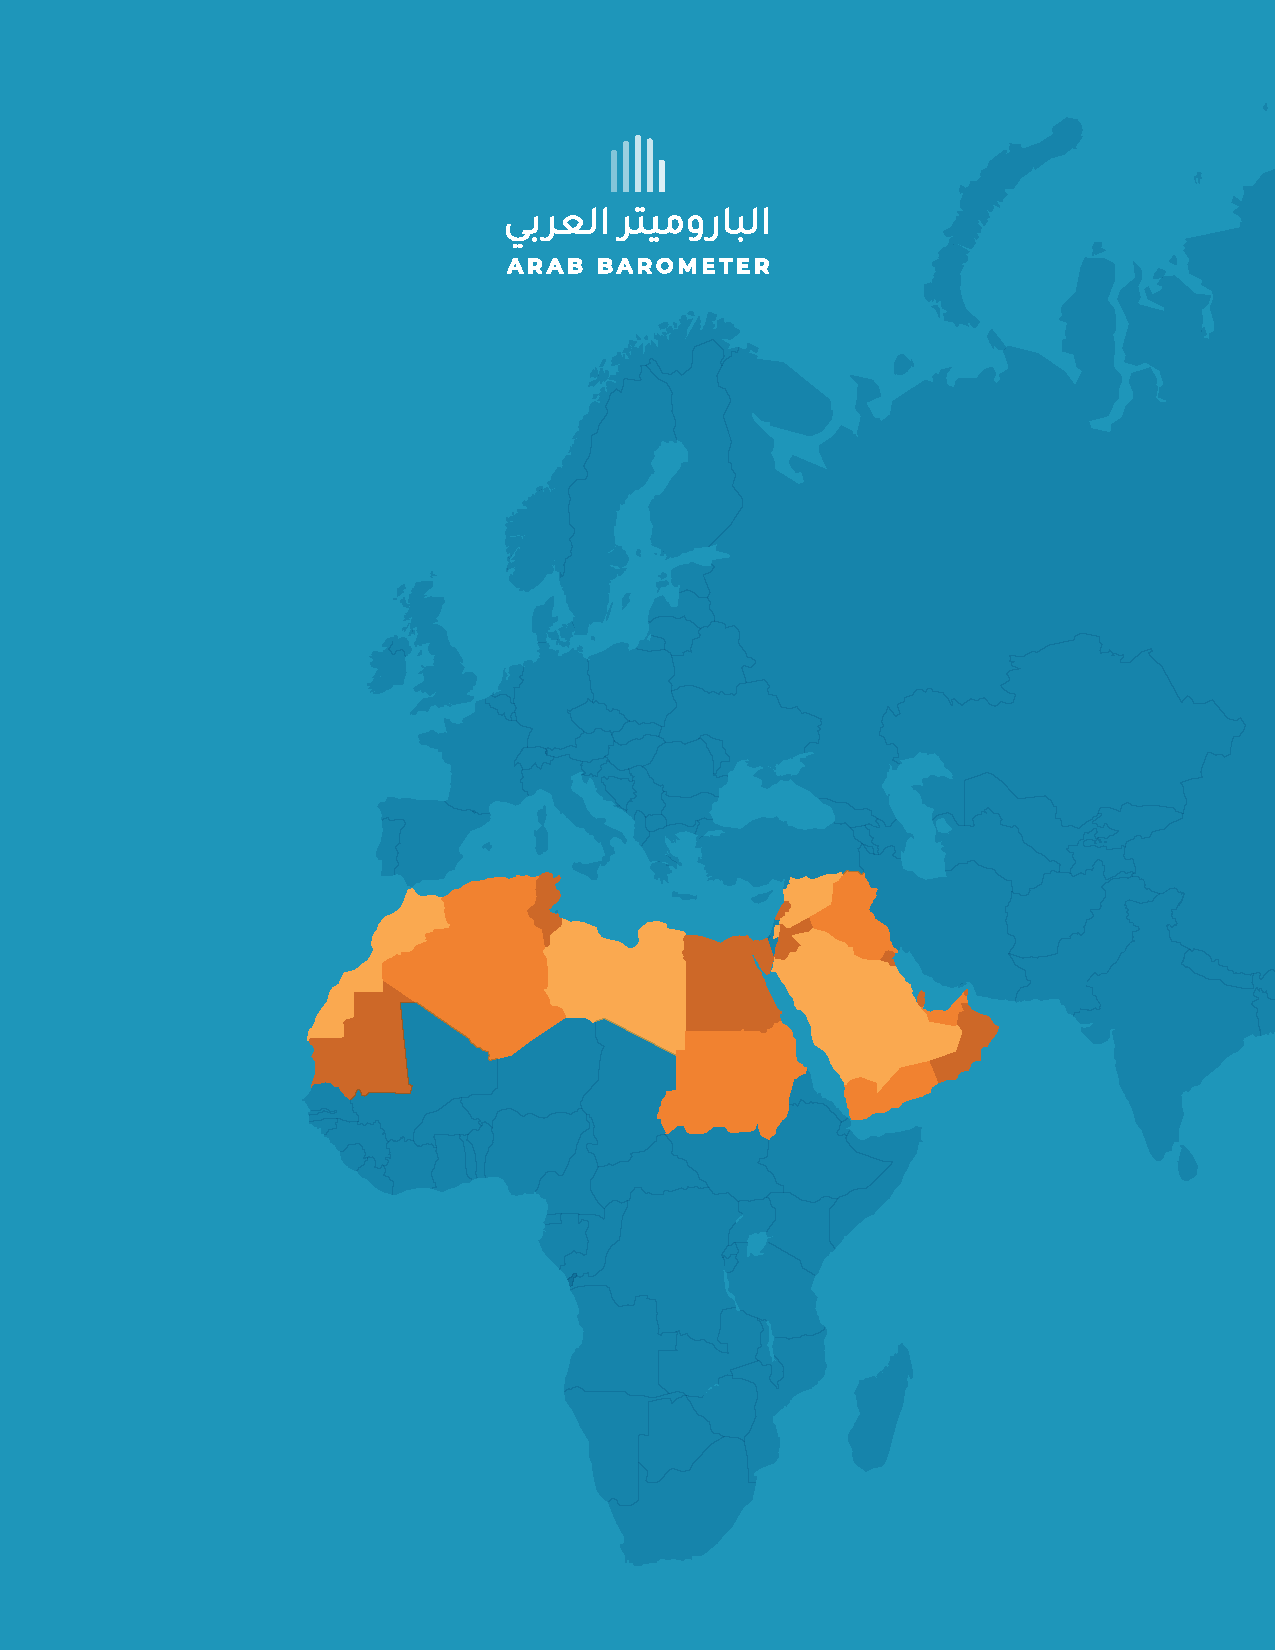
\includegraphics[width=\paperwidth,height=\paperheight]{AB_FrontCover.pdf}
	}%
}
\newgeometry{left=1.5in,right=1.5in,top=1in, bottom=1in}
\pagestyle{empty} 
\vspace*{1in}
\centering
\textbf {\LARGE \color{white} 	\href{http://www.arabbarometer.org/about}{عن الباروميتر العربي}} \\
\vspace*{0.2in}
\normalsize \color{white}{الباروميتر العربي هو شبكة بحثية مستقلة وغير حزبيّة، تقدم نظرة ثاقبة عن الإتجاهات والقيم الإجتماعية والسياسية والإقتصادية للمواطنين العاديين في العالم العربي. 
 \\
	\vspace*{0.2in}
تقوم الشبكة بإجراء إستطلاعات للرأي العام في الشرق الأوسط وشمال أفريقيا ذات مستوى عالٍ من الجودة والمصداقية منذ عام 2006 \\
	\vspace*{0.2in}
نحن أضخم مستودع للبيانات المتاحة في متناول العامة حول آراء الرجال والنساء في المنطقة. تمنح نتائج استطلاعاتنا فسحة للمواطنين العرب للتعبير عن احتياجاتهم واهتماماتهم.
 \\	
	\vspace*{4.1in}	
	\begin{tabular}{R {2.2in} R {2in} R {2in}}
		\Huge \color{abblue}{
			\href{http://www.arabbarometer.org}{..........} }&
		\Huge \color{abblueD}{\href{http://www.facebook.com/arabbarometer/}{..........} }&	
		\Huge \color{abblue}{
			\href{https://twitter.com/arabbarometer}{..........}}\\
	\end{tabular}

\end{document}